% Lernblatt Terme – gebaut aus der Aufgabenbank (bank/terme) nach Prompt
% v5.1, Vorbild Muster 4 (bau/terme/muster-2026-10-01/muster4.tex).
% Blattfolge der Mappe (Katalog 9e85c1e): 1 Zusammenfassen, 2 Malnehmen,
% 3 Klammern auflösen, 4 Ausklammern, 5 Termwerte, 6 Terme aufstellen;
% Blatt 0 davor, „Zum Schluss“ und Lösungen dahinter.
% Quelle je Teilaufgabe im Kommentar davor: % <id> = aus der Bank (Auftrag im
% Titel der Nummer; ids nach der Sechs-Einheiten-Bank, Stand Commit 4493f71),
% % GEÄNDERT <id> = Form oder Zahlen geändert, % NEU = nicht in der Bank.
% % pruef: … = Rechenprobe (pruef.py).
\documentclass[11pt]{article}
\usepackage{mathblatt}
\usepackage{multicol}
\usepackage{lastpage}
% Kopf: nur das Thema; Fuß: „Seite n von m“
\pagestyle{fancy}\fancyhf{}\renewcommand{\headrulewidth}{0pt}
\setlength{\headheight}{14pt}
\fancyhead[L]{\small Terme}
\fancyfoot[C]{\small Seite \thepage\ von \pageref{LastPage}}
\raggedright
\makeatletter
% ---------------------------------------------------------------- Satz
\newcommand{\vorgerechnet}[1]{\textcolor{gray!70}{#1}}
\newcommand{\einheit}[2]{\par\Needspace*{0.33\textheight}\addvspace{16pt}%
  \noindent{\Large\bfseries\ifblank{#1}{}{#1\hspace{0.6em}}#2}\par\nobreak\vspace{2pt}%
  \gappto\mblsg{\lsgeinheit{\ifblank{#1}{}{#1\ }#2}}}
\newsavebox{\nrbox}\newlength{\nrhoehe}
\newcommand{\nrtitel}[1]{\noindent\hangindent1.6em\hangafter1%
  \makebox[1.6em][l]{\textbf{\theaufgabe.}}#1\par\vspace{1pt}}
\newenvironment{nr}[2][]{\refstepcounter{aufgabe}\setcounter{teil}{0}%
  \def\nrart{#1}%
  \ifx\nrart\@empty
    \begin{lrbox}{\nrbox}\begin{minipage}[t]{\linewidth}\raggedright
    \setlength{\parskip}{0pt}\nrtitel{#2}%
  \else
    \par\addvspace{11pt}\Needspace*{8\baselineskip}\nrtitel{#2}%
  \fi}%
 {\ifx\nrart\@empty
    \end{minipage}\end{lrbox}%
    \setlength{\nrhoehe}{\dimexpr\ht\nrbox+\dp\nrbox\relax}%
    \par\addvspace{11pt}\Needspace*{\nrhoehe}\noindent\usebox{\nrbox}\par
  \else\par\fi}
\newcommand{\teilmarke}{\stepcounter{teil}\makebox[1.6em][r]{\alph{teil})\hspace{0.35em}}}
\newcommand{\marke}[1]{\ifblank{#1}{}{\hfill{\footnotesize #1}}}
\newlength{\feldbreite}\setlength{\feldbreite}{4.5cm}
\newcommand{\antwort}{\underline{\hspace{\feldbreite}}}
\newcommand{\zeilenluft}{\par\nobreak\vskip 12pt plus 1pt\relax}
\newcommand{\zeilenluftb}{\par\vskip 12pt plus 1pt\relax}
\newlength{\kw}\newlength{\kwmax}
\newcounter{kzahl}\newcounter{kzeile}
\newcommand{\kliste}{}
\newcommand{\kmerke}[2]{\settowidth{\kw}{#1}%
  \ifdim\kw>\kwmax\global\kwmax=\kw\fi\stepcounter{kzahl}\gappto\kliste{#2}}
\newcommand{\kstart}[1]{\global\kwmax=0pt\setcounter{kzahl}{0}\setcounter{kzeile}{0}%
  \gdef\kliste{}\setlength{\feldbreite}{#1}}
\newcommand{\kende}{\par\vspace{3pt}\kliste\par}
\newcommand{\kettezeile}[1]{\stepcounter{kzeile}%
  \ifnum\value{kzeile}>1
    \ifnum\value{kzeile}<4 \zeilenluft
    \else\ifnum\numexpr\value{kzahl}-\value{kzeile}\relax<2 \zeilenluft
    \else\zeilenluftb\fi\fi
  \fi
  \noindent#1\par}
\newenvironment{kette}[1][4.5cm]{\kstart{#1}}{\kende}
\newcommand{\termspalte}[1]{\makebox[\kwmax][l]{$#1 =$}\hspace{0.6em}}
\NewDocumentCommand{\rk}{O{} m m}{\kmerke{$#2 =$}{\kettezeile{\teilmarke\lsgm{#3}%
  \termspalte{#2}\antwort\marke{#1}}}}
\newcommand{\rkv}[2]{\kmerke{$#1 =$}{\kettezeile{\teilmarke\termspalte{#1}%
  \vorgerechnet{$#2$}}}}
\newenvironment{werte}[1][2.8cm]{\kstart{#1}}{\kende}
\newcommand{\wertkopf}[2]{$#1$\hspace{0.8em}für $#2$:}
\NewDocumentCommand{\rw}{O{} m m m}{\kmerke{\wertkopf{#2}{#3}}{\kettezeile{\teilmarke\lsgm{#4}%
  \makebox[\kwmax][l]{\wertkopf{#2}{#3}}\hspace{0.6em}\antwort\marke{#1}}}}
\newcommand{\rwv}[3]{\kmerke{\wertkopf{#1}{#2}}{\kettezeile{\teilmarke
  \makebox[\kwmax][l]{\wertkopf{#1}{#2}}\hspace{0.6em}\vorgerechnet{$#3$}}}}
\NewDocumentCommand{\rt}{O{} m m}{\par\vspace{7pt}\noindent\hangindent1.6em\hangafter1
  \teilmarke\lsgt{#3}#2\nobreak\hspace{0.6em}\underline{\hspace{4cm}}\marke{#1}\par}
\newlength{\kennbreite}\setlength{\kennbreite}{1.6cm}
\NewDocumentCommand{\rtx}{O{} m m}{\par\vspace{7pt}\noindent
  \ifblank{#1}{\parbox[t]{\linewidth}{\raggedright\hangindent1.6em\hangafter1
   \teilmarke\lsgt{#3}#2}}%
  {\parbox[t]{\dimexpr\linewidth-\kennbreite\relax}{\raggedright\hangindent1.6em\hangafter1
   \teilmarke\lsgt{#3}#2}\parbox[t]{\kennbreite}{\raggedleft\footnotesize #1}}\par}
\NewDocumentCommand{\rs}{O{} m m}{\par\vspace{9pt}\noindent
  \teilmarke\lsgt{#3}%
  \ifblank{#1}{\parbox[t]{\dimexpr\linewidth-1.6em\relax}{\raggedright #2}}%
   {\parbox[t]{\dimexpr\linewidth-1.6em-\kennbreite\relax}{\raggedright #2}%
    \parbox[t]{\kennbreite}{\raggedleft\footnotesize #1}}\par\raum}
\newcommand{\raum}{\par\nobreak\vspace{6mm}\noindent\hspace*{1.6em}%
  \rule{0.5\textwidth}{0.4pt}\par\nobreak\vspace{6mm}\noindent\hspace*{1.6em}%
  \rule{0.5\textwidth}{0.4pt}\par}
\newcommand{\kreuzzeile}[1]{\par\vspace{6pt}\noindent\hspace*{1.6em}#1\par}
\renewcommand{\kreuz}[1]{$\square$\,#1\hspace{2.2em}}
\newenvironment{zusammen}{\par\noindent\begin{minipage}{\linewidth}}{\end{minipage}\par}
\newcommand{\figurfelder}[2]{\par\vspace{6pt}\noindent\hspace*{1.6em}%
  $\vcenter{\hbox{#1}}$\hspace{1.5em}\begin{tabular}[c]{@{}l@{\hspace{0.5em}}l@{}}#2\end{tabular}\par}
% Merkkasten: schmaler Rahmen, je Zeile ein Fall (Stichwort fett, Beispiel,
% Ergebnis fett), zuletzt „Wichtig:“
\newcommand{\merk}[1]{\par\nobreak\vspace{5pt}\noindent
  \fcolorbox{black!60}{white}{\parbox{\dimexpr\linewidth-2\fboxsep-2\fboxrule\relax}{%
  \raggedright\setlength{\parskip}{1.5pt}#1}}\par\vspace{2pt}}
\newcommand{\mz}[2]{\textbf{#1} #2\par}
% ---------------------------------------------------------------- Lösungen
\newcommand{\mblsg}{}
\newcommand{\lsgm}[1]{\lsgt{$#1$}}
\newcommand{\lsgextra}{}
\newcommand{\lsgt}[1]{\xappto\mblsg{\noexpand\lz{\theaufgabe}{\alph{teil}}}%
  \xappto\mblsg{{\unexpanded{#1}\unexpanded\expandafter{\lsgextra}}}%
  \gdef\lsgextra{}}
\newcommand{\falsch}[1]{\gdef\lsgextra{\quad{\footnotesize falsch $\rightarrow$ Nr.~#1}}}
\newcommand{\falschk}[1]{\gappto\kliste{\falsch{#1}}}
\newcommand{\lzletzte}{0}
\newcommand{\lz}[3]{\par\noindent\hangindent3.4em\hangafter1
  \ifnum#1=\lzletzte\relax\makebox[1.8em][l]{}\else\makebox[1.8em][l]{\textbf{#1}}\fi
  \gdef\lzletzte{#1}%
  \makebox[1.6em][l]{\ifx&#2&\else#2)\fi}#3\par}
\newcommand{\lsgeinheit}[1]{\par\addvspace{4pt}\noindent{\bfseries #1}\par}
\makeatother

\begin{document}
\setlength{\parskip}{0pt}

% =================================================================== Blatt 0
\einheit{}{Das kennst du schon}
\noindent
\begin{minipage}[t]{0.48\linewidth}
\begin{nr}{Plus und Minus}
\begin{kette}[2cm]
% terme-zone-f1-v1
\rk{4 - 9}{-5}
% terme-zone-f1-v4
\rk{-6 - 4}{-10}
% terme-zone-f1-v3
\rk{-2{,}5 + 1}{-1{,}5}
\end{kette}
\end{nr}
\begin{nr}{Mal mit Vorzeichen}
\begin{kette}[2cm]
% terme-zone-f2-v1
\rk{(-5) \cdot 2}{-10}
% terme-zone-f2-v4
\rk{(-4) \cdot (-5)}{20}
% terme-zone-f2-v3
\rk{(-0{,}5) \cdot 8}{-4}
\end{kette}
\end{nr}
\end{minipage}\hfill
\begin{minipage}[t]{0.48\linewidth}
\begin{nr}{Dezimalzahlen und Brüche}
\begin{kette}[2cm]
% terme-zone-f3-v2
\rk{\frac{1}{2} + \frac{1}{4}}{\frac{3}{4}}
% terme-zone-f3-v3
\rk{0{,}5 - 1{,}5}{-1}
% NEU
\rk{-0{,}6 - 0{,}9}{-1{,}5}
\end{kette}
\end{nr}
\begin{nr}{Punkt vor Strich}
\begin{kette}[2cm]
% terme-zone-f4-v1
\rk{5 + 2 \cdot 4}{13}
% terme-zone-f4-v3
\rk{6 - 4 \cdot 2{,}5}{-4}
% NEU
\rk{4 - 3 \cdot (-2)}{10}
\end{kette}
\end{nr}
\end{minipage}

% =================================================================== Einheit 1
\einheit{1}{Terme zusammenfassen}
\merk{\mz{Gleiche Variablen:}{Vorzahlen addieren, die Variable bleibt: $3x + 5x = \mathbf{8x}$}
\mz{Zahl ohne Variable bleibt:}{$7a - 2a + 4 = \mathbf{5a + 4}$}
\mz{Hochzahl zählt mit:}{$x^2 + 3x$ \textbf{bleibt so}}
\mz{Wichtig:}{$3x + 4$ ist nicht $7x$; $x$ hat die Vorzahl 1, also $x + 6x = 7x$, nicht $6x$.}}

\begin{nr}[b]{Fasse zusammen.}\label{nr:zus}
\begin{kette}
% terme-e1-k4-s1-v3
\rk{7x + 5x}{12x}
% terme-e1-k4-s2-v1
\rk{9x - 4x}{5x}
% terme-e1-k4-s4-v1
\rk{5x + 3 + 2x}{7x + 3}
% terme-e1-k4-s5-v2
\rk{2x + 5y + 4x}{6x + 5y}
% NEU
\rk{-4y + 1{,}5 - y - 3{,}5}{-5y - 2}
% terme-e1-k4-s10-v1
\rk{4x^2 + 5x + 2x^2}{6x^2 + 5x}
% NEU
\rk[GYM]{\frac{2}{3}a + 4ab - \frac{1}{6}a - 7ab + b}{\frac{1}{2}a - 3ab + b}
\end{kette}
\end{nr}

\begin{nr}{Abschluss}
% GEÄNDERT terme-e1-k5-s3-v2 (Form: Feld neben der Figur)
% pruef: 3*a + 2*a + 4*a == 9*a
\begin{zusammen}
\rtx{Die Figur zeigt ein Dreieck (Maße in cm). Schreibe einen Term für den Umfang und fasse ihn zusammen.}{$3a + 2a + 4a = 9a$}
\figurfelder{\dreieck{(0,0)}{(3.2,0)}{(1.1,1.0)}{3a}{2a}{4a}{}{}{}}{& \underline{\hspace{4cm}}}
\end{zusammen}
% NEU
\rtx{Welcher Term passt zu $5a + 3 + 2a$? Kreuze an.}{$7a + 3$}
\kreuzzeile{\kreuz{$10a$}\kreuz{$7a + 3$}\kreuz{$3a + 7$}\kreuz{$7a$}}
% terme-e1-k4-s15-v1
% pruef: 8*a - 2*a**2 - 5*a == 3*a - 2*a**2
% pruef: 3*3 - 2*3**2 == -9
\rs[P10 ’25]{Vereinfache den Term $8a - 2a^2 - 5a$ und berechne seinen Wert für $a = 3$.}{$3a - 2a^2$; für $a = 3$: $-9$}
\end{nr}

% =================================================================== Einheit 2
\einheit{2}{Terme malnehmen}
\merk{\mz{Zahl mal Term:}{Zahlen mal Zahlen, die Variable bleibt: $3 \cdot 4x = \mathbf{12x}$}
\mz{Term mal Term:}{Variablen mal Variablen gibt eine Hochzahl: $2x \cdot 3x = \mathbf{6x^2}$}
\mz{Zwei Variablen:}{$3a \cdot 2b = \mathbf{6ab}$}
\mz{Wichtig:}{$x \cdot x$ ist $x^2$, nicht $2x$; beim Malnehmen zählen die Vorzeichen wie bei Zahlen.}}

\begin{nr}[b]{Multipliziere.}\label{nr:mal}
\begin{kette}
% terme-e2-k1-s1-v3
\rk{5 \cdot 6x}{30x}
% terme-e2-k1-s2-v3
\rk{2z \cdot 8}{16z}
% terme-e2-k1-s3-v3
\rk{z \cdot 7z}{7z^2}
% terme-e2-k1-s4-v1
\rk{(-4) \cdot 5x}{-20x}
% terme-e2-k1-s5-v3
\rk{5b \cdot 2c}{10bc}
% terme-e2-k1-s11-v3
\rk{3y \cdot (-5x)}{-15xy}
% NEU
\rk{\frac{3}{5}a \cdot 10b \cdot (-2a)}{-12a^2b}
% NEU
\rk[GYM]{2a \cdot 4b - 3ab + a \cdot (-2b)}{3ab}
\end{kette}
\end{nr}

\begin{nr}{Abschluss}
\begin{kette}
% NEU
\rk{(-3a) \cdot a \cdot (-2a)}{6a^3}
\end{kette}
% NEU
% pruef: 4*(2*x + x + 3) == 12*x + 12
% pruef: 2*x*x*3 == 6*x**2
\begin{zusammen}
\rtx{Der Quader hat die Kantenlängen $2x$, $x$ und $3$ (in cm). Gib Terme für die Summe aller zwölf Kanten und für das Volumen an und vereinfache.}{Kanten: $4 \cdot (2x + x + 3) = 12x + 12$; Volumen: $6x^2$}
\figurfelder{\quader{2.4}{1.2}{1.4}{2x}{x}{3}}{Kantensumme: & \underline{\hspace{4cm}} \\[8mm]
Volumen: & \underline{\hspace{4cm}}}
\end{zusammen}
% NEU
\rs{Mia rechnet $3b \cdot 2b = 6b$. Stimmt das? Begründe.}{Nein: $b \cdot b = b^2$, also $6b^2$}
\end{nr}

% =================================================================== Einheit 3
\einheit{3}{Klammern auflösen}
\merk{\mz{Plus vor der Klammer:}{Klammer weglassen: $a + (b - c) = \mathbf{a + b - c}$}
\mz{Minus vor der Klammer:}{alle Vorzeichen drehen: $a - (b - c) = \mathbf{a - b + c}$}
\mz{Zahl mal Klammer:}{jedes Glied malnehmen: $3 \cdot (x + 4) = \mathbf{3x + 12}$}
\mz{Wichtig:}{Bei der Minusklammer dreht sich jedes Vorzeichen in der Klammer, nicht nur das erste: $-(x - 4) = -x + 4$.}}

\begin{nr}[b]{Plusklammer und Minusklammer – löse auf.}\label{nr:pm}
\begin{kette}
% terme-e3-k2-s1-v3 (vorgerechnet)
\rkv{5a + (2b - 4)}{5a + 2b - 4}
% terme-e3-k2-s1-v5
\rk{5a + (2b - 8)}{5a + 2b - 8}
% terme-e3-k2-s3-v1
\rk{5a - (2b + 4)}{5a - 2b - 4}
% terme-e3-k2-s4-v3
\rk{10 - (3a - 4b + 6c)}{10 - 3a + 4b - 6c}
% NEU
\rk{3{,}5 - (-2x + 1{,}5y - 0{,}5)}{2x - 1{,}5y + 4}
% NEU
\rk{(2x^2 - 3x) - (x^2 + 4x) - (-5x)}{x^2 - 2x}
\end{kette}
\end{nr}

\begin{nr}[b]{Mal Klammer – löse die Klammer auf.}
\begin{kette}
% GEÄNDERT terme-e3-k3-s1-v3 (Form: ohne Tabelle; vorgerechnet)
\rkv{7 \cdot (b + 3)}{7 \cdot b + 7 \cdot 3 = 7b + 21}
% GEÄNDERT terme-e3-k3-s1-v1 (Form: ohne Tabelle)
\rk{5 \cdot (x + 3)}{5x + 15}
% terme-e3-k3-s2-v2
\rk{-3 \cdot (a - 7)}{-3a + 21}
% NEU
\rk{4a \cdot (2a - 3)}{8a^2 - 12a}
% NEU
\rk{(2x - 5y + 3) \cdot (-3)}{-6x + 15y - 9}
% NEU
\rk{\frac{1}{2}y \cdot (6y - 8 + 4x)}{3y^2 - 4y + 2xy}
\end{kette}
\end{nr}

\begin{nr}[b]{Löse die Klammern auf und fasse zusammen.}\label{nr:kz}
\begin{kette}
% terme-e3-k4-s1-v2 (vorgerechnet)
\rkv{9a - (4a + 3)}{9a - 4a - 3 = 5a - 3}
% terme-e3-k4-s1-v1
\rk{5x + 2 \cdot (x + 6)}{7x + 12}
% terme-e3-k4-s8-v2
\rk{5 \cdot (a + 3) - 2 \cdot (a - 1)}{3a + 17}
% NEU
\rk{2a \cdot (a + 4) - a \cdot (3 - a)}{3a^2 + 5a}
% NEU
\rk{6x - [\,4 - 2 \cdot (x - 3)\,]}{8x - 10}
% NEU
\rk[GYM]{2x - \{\,3y - [\,2x - (y - x)\,]\,\}}{5x - 4y}
% NEU
\rk[GYM]{-3a \cdot (2b - a) + 2 \cdot (ab - a^2) - a \cdot (-b)}{a^2 - 3ab}
% NEU
\rk[GYM]{\frac{1}{3} \cdot (9x - 6y) - \frac{1}{2} \cdot (4y - 2x)}{4x - 4y}
\end{kette}
\end{nr}

\begin{nr}{Abschluss}
\begin{kette}
% NEU
\rk{8y - (3y - 5) + 2 \cdot 3y}{11y + 5}
\end{kette}
% terme-e3-k4-s4-v3
% pruef: 2.5*(20 + x) == 50 + 2.5*x
% pruef: 50 + 2.5*4 == 60
\rs{Ein Muffin kostet 2,50 €. Für eine Feier werden 20 Muffins bestellt und noch $x$ Muffins dazu. Schreibe den Preis in Euro als Term mit Klammer. Löse die Klammer auf. Was kosten die Muffins bei $x = 4$?}{$2{,}50 \cdot (20 + x) = 50 + 2{,}50x$; $60\,€$}
% terme-e3-k5-s2-v2
\rs{Kai sagt: „Bei $15 - (x - 3)$ muss ich nur das Vorzeichen von $x$ umdrehen. Das ergibt $15 - x - 3$.“ Stimmt das? Begründe.}{Nein: Minus vor der Klammer dreht jedes Vorzeichen, richtig ist $15 - x + 3 = 18 - x$}
\end{nr}

% =================================================================== Einheit 4
\einheit{4}{Ausklammern}
\merk{\mz{Zahl ausklammern:}{$6x + 9 = \mathbf{3 \cdot (2x + 3)}$}
\mz{Variable ausklammern:}{$4a^2 + 2a = \mathbf{2a \cdot (2a + 1)}$}
\mz{Probe:}{ausmultiplizieren, der Anfangsterm muss herauskommen: $2a \cdot 2a + 2a \cdot 1 = \mathbf{4a^2 + 2a}$}
\mz{Wichtig:}{Ist ein Glied selbst der Faktor, bleibt in der Klammer eine 1: $8x - 8 = 8 \cdot (x - 1)$, nicht $8 \cdot x$.}}

\begin{nr}[b]{Klammere den größten gemeinsamen Faktor aus; bei g) schreibe die Probe dahinter.}\label{nr:aus}
\begin{kette}[6cm]
% terme-e4-k2-s1-v5 (vorgerechnet)
\rkv{5x + 40}{5 \cdot x + 5 \cdot 8 = 5 \cdot (x + 8)}
% terme-e4-k2-s1-v2
\rk{5x + 25}{5 \cdot (x + 5)}
% terme-e4-k2-s2-v3
\rk{b^2 + 9b}{b \cdot (b + 9)}
% terme-e4-k2-s3-v3
\rk{10y^2 + 4y}{2y \cdot (5y + 2)}
% terme-e4-k2-s4-v1
\rk{6x + 6}{6 \cdot (x + 1)}
% NEU
\rk{-8a^2b + 12ab^2 - 4ab}{-4ab \cdot (2a - 3b + 1)}
% terme-e4-k2-s14-v3
\rk{16xy + 4y^2 - 8y}{4y \cdot (4x + y - 2) = 16xy + 4y^2 - 8y}
% NEU
\rk[GYM]{3x \cdot (a - b) + 2y \cdot (a - b)}{(a - b) \cdot (3x + 2y)}
\end{kette}
\end{nr}

\begin{nr}{Abschluss}
% GEÄNDERT terme-e4-k2-s7-v1 (Form: Figur mit Feldern)
% pruef: 4*x + 4*6 == 4*(x + 6)
\begin{zusammen}
\rtx{Flächeninhalt der Figur (Maße in cm) als Summe der Teilflächen und als Produkt mit Klammer:}{Summe: $4x + 24$; Produkt: $4 \cdot (x + 6)$}
\figurfelder{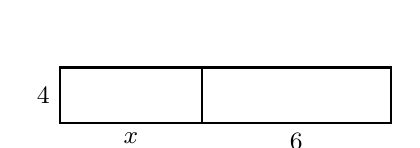
\begin{tikzpicture}[line width=0.8pt]
\draw (0,0) rectangle (1.8,0.7); \draw (1.8,0) rectangle (4.2,0.7);
\node[left,font=\small] at (0,0.35) {$4$};
\node[below,font=\small] at (0.9,0) {$x$};
\node[below,font=\small] at (3.0,0) {$6$};
\end{tikzpicture}}{Summe: & \underline{\hspace{3.2cm}}\quad Produkt: \underline{\hspace{3.2cm}}}
\end{zusammen}
% GEÄNDERT terme-e4-k2-s10-v3 (Auftrag gekürzt)
% pruef: 0.25*(14 + 18 + 8) == 10
\rs{Drei Bücher kosten 14 €, 18 € und 8 €, Rabatt 25 \%. Mila rechnet $0{,}25 \cdot 14 + 0{,}25 \cdot 18 + 0{,}25 \cdot 8$, Tarek $0{,}25 \cdot (14 + 18 + 8)$. Ergeben beide denselben Rabatt? Begründe.}{Ja: $0{,}25$ ist ausgeklammert, beide ergeben $10\,€$}
% NEU
\rtx{Welcher Term ist gleichwertig zu $12x - 18$? Kreuze an.}{$6 \cdot (2x - 3)$}
\kreuzzeile{\kreuz{$6 \cdot (2x - 18)$}\kreuz{$6 \cdot (2x - 3)$}\kreuz{$12 \cdot (x - 18)$}\kreuz{$2 \cdot (6x - 18)$}}
\end{nr}

% =================================================================== Einheit 5
\einheit{5}{Termwerte berechnen}
\merk{\mz{Einsetzen:}{die Zahl für die Variable, dann Punkt vor Strich: $2 + 5x$ für $x = 3$: $2 + 5 \cdot 3 = \mathbf{17}$}
\mz{Negative Zahl:}{in Klammern einsetzen: $3x^2$ für $x = -2$: $3 \cdot (-2)^2 = \mathbf{12}$}
\mz{Wichtig:}{$(-2)^2$ ist $4$, nicht $-4$; ohne Klammer geht das Vorzeichen verloren.}}

\begin{nr}[b]{Berechne den Wert des Terms.}\label{nr:wert}
\begin{werte}
% terme-e5-k1-s2-v2 (vorgerechnet)
\rwv{10 - 3x}{x = -2}{10 - 3 \cdot (-2) = 16}
% terme-e5-k1-s1-v1
\rw{4x - 3}{x = 5}{17}
% terme-e5-k1-s2-v1
\rw{2x + 9}{x = -3}{3}
% NEU
\rw{x^2 - 3x}{x = -4}{28}
% NEU
\rw{8x^2 - 2x}{x = -\frac{1}{2}}{3}
% NEU
\rw{\frac{1}{3}a - 2b}{a = 9,\ b = -\frac{3}{4}}{4{,}5}
% NEU
\rw{3 \cdot (x - y)^2 - xy}{x = -2,\ y = 1}{29}
\end{werte}
\end{nr}

% =================================================================== Einheit 6
\einheit{6}{Terme aufstellen}
\merk{\mz{Vermindert um:}{„$x$ um 5 vermindert“: $\mathbf{x - 5}$}
\mz{Das Mehrfache einer Summe:}{„das Doppelte der Summe aus $x$ und 5“: $\mathbf{2 \cdot (x + 5)}$, mit Klammer}
\mz{Aus der Figur:}{Umfang eines Rechtecks mit den Seiten $a$ und 3: $a + 3 + a + 3 = \mathbf{2a + 6}$}
\mz{Wichtig:}{„5 vermindert um $x$“ ist $5 - x$, nicht $x - 5$; ohne Klammer wird nur $x$ verdoppelt.}}

\begin{nr}[b]{Schreibe einen Term.}\label{nr:auf}
% terme-e6-k1-s2-v2
% pruef: 2*x - 5 == 2*x - 5
\rt{Das Doppelte einer Zahl $x$ wird um 5 vermindert.}{$2x - 5$}
% terme-e6-k1-s2-v1
% pruef: 3*x + 8 == 3*x + 8
\rt{Das Dreifache einer Zahl $x$ wird um 8 vergrößert.}{$3x + 8$}
% GEÄNDERT terme-e6-k1-s3-v2 (Form: Feld neben der Figur)
% pruef: x + x + 6 == 2*x + 6
\begin{zusammen}
\rtx{Umfang des Dreiecks (Maße in cm):}{$x + x + 6 = 2x + 6$}
\figurfelder{\dreieck{(0,0)}{(3.2,0)}{(1.6,1.4)}{x}{x}{6}{}{}{}}{& \underline{\hspace{4cm}}}
\end{zusammen}
% terme-e6-k1-s4-v3
% pruef: 6*p + 2*q == 6*p + 2*q
\rt{Eine Kiste Äpfel wiegt $p$ kg, eine Kiste Birnen $q$ kg. Auf dem Wagen stehen 6 Kisten Äpfel und 2 Kisten Birnen. Wie schwer sind alle Kisten?}{$6p + 2q$}
% GEÄNDERT terme-e6-k1-s5-v3 (Auftrag gekürzt)
% pruef: x + x + 2 + 2*x == 4*x + 2
\rt{Umfang des Dreiecks mit den Seiten $x$, $x + 2$ und $2x$, zusammengefasst:}{$4x + 2$}
% terme-e6-k1-s6-v3
% pruef: (5*x + 3)/2 == (5*x + 3)/2
\rt{Die Summe aus dem Fünffachen einer Zahl $x$ und 3 wird halbiert.}{$(5x + 3) : 2$}
% terme-e6-k1-s10-v4
\rtx[P10 ’17]{Das Doppelte einer Zahl $x$ wird um neun vermindert. Kreuze den passenden Term an.}{$2x - 9$}
\kreuzzeile{\kreuz{$2 \cdot (x - 9)$}\kreuz{$9 - 2x$}\kreuz{$2x - 9$}\kreuz{$2x - 9x$}}
% terme-e6-k1-s10-v1
\rtx[P10 ’23]{Die Differenz aus dem Dreifachen einer Zahl $x$ und 7 wird verdoppelt. Kreuze den passenden Term an.}{$2 \cdot (3x - 7)$}
\kreuzzeile{\kreuz{$(3x - 7) : 2$}\kreuz{$3x : 7 \cdot 2$}\kreuz{$2 \cdot (3x - 7)$}\kreuz{$3x - 7 \cdot 2$}}
\end{nr}

\begin{nr}{Abschluss}
% NEU
% pruef: x + x - 3 == 2*x - 3
\rt{Lea ist $x$ Jahre alt, ihr Bruder 3 Jahre jünger. Beide zusammen:}{$x + x - 3 = 2x - 3$}
% terme-e6-k1-s7-v1
% pruef: 11 + 0.3*150 == 56
\rs{Ein Stromtarif kostet 11 € Grundpreis im Monat und 0,30 € je Kilowattstunde. Stelle einen Term für die Monatskosten in Euro bei $n$ Kilowattstunden auf. Was kostet ein Monat mit 150 Kilowattstunden?}{$11 + 0{,}30n$; $56\,€$}
% terme-e6-k3-s1-v2
% pruef: 2*(x + 7) == 2*x + 14
\rs{Jonas soll zu „das Doppelte der Summe aus einer Zahl $x$ und 7“ einen Term schreiben. Er schreibt $2 \cdot (x + 7)$. Stimmt das? Begründe.}{Ja: erst die Summe $x + 7$, dann verdoppeln – dafür braucht es die Klammer}
\end{nr}

% =================================================================== Zum Schluss
% Je Einheit eine Teilaufgabe mittlerer Höhe (a–f, gemischt), dann zwei
% höhere (g GYM wie Nr. kz f, h P10 ’25 wie Nr. 6 c); Lösungen mit „falsch → Nr. n“.
\par\addvspace{10pt}
\begin{nr}{Zum Schluss}
\begin{kette}
% NEU (Einheit 3)
\falschk{\ref{nr:kz}}
\rk{2 \cdot (3a - 4) - (a - 5)}{5a - 3}
% NEU (Einheit 1)
\falschk{\ref{nr:zus}}
\rk{3a - 5b + 2 - 7a + b}{-4a - 4b + 2}
% NEU (Einheit 2)
\falschk{\ref{nr:mal}}
\rk{2x \cdot (-4xy)}{-8x^2y}
\end{kette}
\par\vspace{6pt}
\begin{werte}
% NEU (Einheit 5)
\falschk{\ref{nr:wert}}
\rw{6 - 2x^2}{x = -1{,}5}{1{,}5}
\end{werte}
% NEU (Einheit 4)
% pruef: 4*x*(3*y - 2) == 12*x*y - 8*x
\falsch{\ref{nr:aus}}
\rt{Klammere aus: \ $12xy - 8x$}{$4x \cdot (3y - 2)$}
% NEU (Einheit 6)
% pruef: 20 + 7*x == 20 + 7*x
\falsch{\ref{nr:auf}}
\rt{Eine Kletterhalle verlangt 20 € Jahresbeitrag und 7 € je Besuch. Stelle einen Term für die Kosten in Euro bei $x$ Besuchen auf.}{$20 + 7x$}
\par\vspace{6pt}
\begin{kette}
% NEU (GYM, wie Nr. kz f)
\falschk{\ref{nr:pm}, \ref{nr:kz}}
\rk[GYM]{3a - \{\,b - [\,2a - (3b - a)\,]\,\}}{6a - 4b}
\end{kette}
% GEÄNDERT terme-e1-k4-s15-v2 (Zahlen; wie Nr. 6 c, Original 2025-GYM-B2a)
% pruef: 7*c - 2*c**2 - 4*c == 3*c - 2*c**2
% pruef: 3*(-3) - 2*(-3)**2 == -27
\falsch{\ref{nr:zus}, \ref{nr:wert}}
\rs[P10 ’25]{Vereinfache den Term $7c - 2c^2 - 4c$ und berechne seinen Wert für $c = -3$.}{$3c - 2c^2$; für $c = -3$: $-27$}
\end{nr}

% =================================================================== Lösungen
\clearpage
\noindent{\Large\bfseries Lösungen}\par\vspace{2pt}
\begin{multicols}{2}\raggedright\small\linespread{0.96}\selectfont
\mblsg
\end{multicols}
\end{document}
